%%%%%%%%%%%%%%%%%%%%%%%%%%%%%%%%%%%%%%%%%%%%%%%%%%%%%%%%%%%%%%
%% Sample document for using the latex class rrlab.cls      %%
%% with information on creating scientific documents.       %%
%%                                                          %%
%% main file: howto.tex                                     %%
%% Author: Jochen Hirth (j_hirth@informatik.uni-kl.de)      %%
%% Author: Tobias Luksch (luksch@informatik.uni-kl.de)      %%
%% Author: Axel Vierling (vierling@cs.rptu.de)              %%
%% Date: July 2003                                          %%
%%                                                          %%
%% Last modified December 2023                              %%
%%%%%%%%%%%%%%%%%%%%%%%%%%%%%%%%%%%%%%%%%%%%%%%%%%%%%%%%%%%%%%

% Definition of the document class (rrlab.cls) with optional parameters
% Different document types:
%   Parameter [thesis] To create a master's or bachelor's thesis
%   Parameter [report] To create a report, no "chapter" only "section" can be used to create project or seminar reports etc.
%                      The command \RRLABmaktetitle can be used to create a paper-like header (e.g. for seminar papers).
%                      The use with \RRLABtitlepage and \RRLABpagenumbers is suitable for applications, reports etc.
%   Parameter [diss] Create a dissertation for submission to the department
%   Parameter [summary] To create the summary of the dissertation to inform the faculty that the PhD process has nearly been completed
%   Parameter [dissfinal] Creating a dissertation for submission to the publisher
% Language options:
%   Parameter [de,en] Language, default is [en]
%   Parameter [latin1] sets input encoding to latin1, default is utf8
% Screen presentations:
%   Parameter [colorlinks] recommended for screen presentation; can be used to switch on the colored links when building with 'pdflatex'
%   Parameter [rgbcolor] sets the color coding to RGB (recommended for screen presentation); CMYK is set by default (for printing)
% Misc Options
%   Parameter [external] If your thesis was done externally, you can choose this option and must give the name of the institution with \RRLABinstitution{}
%   Parameter [draft] Omits title page, table of contents, index, etc. and marks overfull boxes
%   Parameter [boldauthor] highlights the author defined in the file 'bold_author.bib' in the bibliography.
%   Parameter [relaxed] allows slightly less attractive spacing for automatic line breaks
%   Parameter [icsecondpage] 'image correction for 2nd page' makes a binding correction for the 2nd page that corresponds to the red cover pages for bachelor and master theses,
%                             This is helpful if you do not want to print the title of the thesis on the cover page
%                             (there is also a template for this), but want to cut out the title field. Then the title
%                             on the 2nd page fits exactly into this window.


\documentclass[thesis]{template/rrlab}

% First some relevant Information for the work.
% This information is mandatory. Please use the predefined macros 

% Title of the work:
\RRLABtitle{Information on how to create a scientific work with \LaTeX}

% Author of the work:
\RRLABauthor{Jochen Hirth, \RRLABand Tobias Luksch, \RRLABand Axel Vierling}

% Type of the work (e.g. Master Thesis, Project report, Seminar report, Dissertation, ...):
\RRLABtype{Documentation}

% Date of issue
\RRLABinception{1. September 1907}

% Date of submission
\RRLABsubmission{\today}

% First reviewer
\RRLABfirstreviewer{Prof. Dr. Karsten Berns}

% Only for Project-, Seminar report, Bachelor-, Master thesis
% Supervisor
\RRLABsupervisor{A member of the Robotics Research Lab}

%%%%%%%%%%%%%%%%%%%%%%%%%%%%%%%%%%%%%%%%%%
%The following are only for Dissertation
% Second reviewer
\RRLABsecondreviewer{Someone}
% Desired Title
\RRLABdegree{Doktor-Ingenieur (Dr.-Ing.)}
%
% Date of Defense
\RRLABdefense{somewhen}
%
% Head of committee
\RRLABchair{someone}
%
% Dean
\RRLABdean{someone else}
%%%%%%%%%%%%%%%%%%%%%%%%%%%%%%%%%%%%%%%%%%

%%%%%%%%%%%%%%%%%%%%%%%%%%%%%%%%%%%%%%%%%%%%%%%%%%%%%%%%%%%%
%% If you need additional Packages you can add them
%% to the following packages.tex file
%% Is is advised to add things only there to
%% keep a better overview 
%%%%%%%%%%%%%%%%%%%%%%%%%%%%%%%%%%%%%%%%%%%%%%%%%%%%%%%%%%%%
% needed for \begin{comment}
\usepackage{verbatim}

%%%%%%%%%%%%%%%%%%%%%%%%%%%%%%%%%%%%%%%%%%%%%%%%%%%%%%%%%%%%
%% Macro definitions
%% Here the experienced TeX-User can define their own macros
%% or commands
%%
%% For relevant, commonly used macros and names that are
%% already defined see template/rrlab_macros.tex
%%%%%%%%%%%%%%%%%%%%%%%%%%%%%%%%%%%%%%%%%%%%%%%%%%%%%%%%%%%%
%%%%%%%%%%%%%%%%%%%%%%%%%%%%%%%%%%%%%%%%%%%%%%%%%%%%%%%%%%%%
%% Macro definitions
%% Here the experienced TeX-User can define their own macros
%% or commands
%%
%% For relevant, commonly used macros and names that are
%% already defined see template/rrlab_macros.tex
%%%%%%%%%%%%%%%%%%%%%%%%%%%%%%%%%%%%%%%%%%%%%%%%%%%%%%%%%%%%
%% In the following some helpful macros are given

%%%%%%%%%%%%%%%%%%%%%%%%%%%%%%%%%%%%%%%%%%%%%%%%%%%%%%%%%%%%%%%%%%%%%%%%%%%%%%%%%%%%%%%%%%%%%%%%%%%%%%%%%%%%%
%%
%% Math Stuff
%%
%%%%%%%%%%%%%%%%%%%%%%%%%%%%%%%%%%%%%%%%%%%%%%%%%%%%%%%%%%%%%%%%%%%%%%%%%%%%%%%%%%%%%%%%%%%%%%%%%%%%%%%%%%%%%
% \newtcbtheorem[number within=chapter]{definition}{Definition}
% {label type=definition,float,breakable,colback=white,colframe=TUKred,coltitle=white,fonttitle=\bfseries}
% {def}
% \newtcbtheorem[number within=chapter]{notation}{Notation}
% {label type=notation,float,breakable,colback=white,colframe=TUKred80,coltitle=white,fonttitle=\bfseries}
% {nota}
% \newtcbtheorem[number within=chapter]{principle}{Principle}
% {label type=principle,float,breakable,colback=white,colframe=TUKred60,coltitle=black,fonttitle=\bfseries}
% {princ}
% \newtcbtheorem[number within=chapter]{example}{Example}
% {label type=example,float,breakable,colback=white,colframe=TUKred40,coltitle=black,fonttitle=\bfseries}
% {ex}

% \newtcbtheorem[number within=chapter]{theorem}{Theorem}
% {label type=theorem,float,breakable,colback=white,colframe=TUKblue80,coltitle=white,fonttitle=\bfseries}
% {thm}
% \newtcbtheorem[number within=chapter]{lemma}{Lemma}
% {label type=lemma,float,breakable,colback=white,colframe=TUKblue60,coltitle=black,fonttitle=\bfseries}
% {lem}
% \newtcbtheorem[number within=chapter]{proposition}{Proposition}
% {label type=proposition,float,breakable,colback=white,colframe=TUKblue40,coltitle=black,fonttitle=\bfseries}
% {prop}
% \newtcbtheorem[number within=chapter]{corollary}{Corollary}
% {label type=corollary,float,breakable,colback=white,colframe=TUKblue20,coltitle=black,fonttitle=\bfseries}
% {cor}

%%%%%%%%%%%%%%%%%%%%%%%%%%%%%%%%%%%%%%%%%%%%%%%%%%%%%%%%%%%%%%%%%%%%%%%%%%%%%%%%%%%%%%%%%%%%%%%%%%%%%%%%%%%%%
%%
%% Figures
%%
%%%%%%%%%%%%%%%%%%%%%%%%%%%%%%%%%%%%%%%%%%%%%%%%%%%%%%%%%%%%%%%%%%%%%%%%%%%%%%%%%%%%%%%%%%%%%%%%%%%%%%%%%%%%%
\newcommand{\rrfig}[1]{{figure~\ref{fig:#1}}}
\newcommand{\rrsubfig}[1]{{subfigure~\subref{fig:#1}}}
\newcommand{\rrtable}[1]{{table~\ref{tab:#1}}}

%%%%%%%%%%%%%%%%%%%%%%%%%%%%%%%%%%%%%%%%%%%%%%%%%%%%%%%%%%%%%%%%%%%%%%%%%%%%%%%%%%%%%%%%%%%%%%%%%%%%%%%%%%%%%
%%
%% Color definitions
%%
%%%%%%%%%%%%%%%%%%%%%%%%%%%%%%%%%%%%%%%%%%%%%%%%%%%%%%%%%%%%%%%%%%%%%%%%%%%%%%%%%%%%%%%%%%%%%%%%%%%%%%%%%%%%%

\newcommand{\tukbluename}{blue}
\definecolor{TUKblue}{RGB}{0,95,140} 		%-> 175,141,118
\definecolor{TUKblue80}{RGB}{51,127,163}	%-> 140,113,94
\definecolor{TUKblue60}{RGB}{102,159,186}	%-> 105,84,81
\definecolor{TUKblue40}{RGB}{153,191,209}	%-> 70,56,47
\definecolor{TUKblue20}{RGB}{204,223,232}	%-> 35,28,24
\definecolor{TUKblue5}{RGB}{242,247,249}	%-> 9,7,6

\newcommand{\tukredname}{red}
\definecolor{TUKred}{RGB}{185,40,25}		%-> 70,215,230
\definecolor{TUKred80}{RGB}{199,83,71}          %-> 56,172,184
\definecolor{TUKred60}{RGB}{213,126,117}        %-> 42,129,138
\definecolor{TUKred40}{RGB}{227,169,163}        %-> 28,86,92
\definecolor{TUKred20}{RGB}{241,212,209}        %-> 14,43,46
\definecolor{TUKred5}{RGB}{251,244,245}         %-> 4,11,10

\definecolor{TUKgrey}{RGB}{130,140,150}
\definecolor{TUKgrey15}{RGB}{216,216,216}       %-> 39,39,39

\definecolor{RPTUSlate}{RGB}{080, 114, 137}	%-> 080, 114, 137
\definecolor{RPTUOcean}{RGB}{119, 182, 186}	%-> 119, 182, 186
\definecolor{RPTUNight}{RGB}{004, 044, 088}	%-> 004, 044, 088
\definecolor{RPTUDay}{RGB}{106, 178, 231}	%-> 106, 178, 231
\definecolor{RPTUPetrol}{RGB}{000, 107, 107}	%-> 000, 107, 107
\definecolor{RPTUApple}{RGB}{038, 208, 124}	%-> 038, 208, 124
\definecolor{RPTUPlum}{RGB}{076, 053, 117}	%-> 076, 053, 117
\definecolor{RPTUFuchsia}{RGB}{209, 056, 150}	%-> 209, 056, 150
\definecolor{RPTURaspberry}{RGB}{227, 027, 076} %-> 227, 027, 076
\definecolor{RPTUMango}{RGB}{255, 162, 082}	%-> 255, 162, 082
\definecolor{RPTUBlack}{RGB}{000, 000, 000}	%-> 000, 000, 000
\definecolor{RPTUWhite}{RGB}{255, 255, 255}	%-> 255, 255, 255


\newcommand{\latexklasse}{\texttt{rrlab.cls}}

%%%%%%%%%%%%%%%%%%%%%%%%%%%%%%%%%%%%%%%%%%%%%%%%%%%%%%%%%%%%
%% Document Environment. 
%% Here the actual document starts
%%%%%%%%%%%%%%%%%%%%%%%%%%%%%%%%%%%%%%%%%%%%%%%%%%%%%%%%%%%%
\begin{document}
% Comment the following commands out depending on your needs

% Generate a title page. The parameter can e.g. be an Image
% or additional text that shows up in the middle of the page
% Additionally the date is forwarded
% For Dissertations: Neither the date nor the title image is needed and therefore not shown
\RRLABtitlepage{An image or something else, usage: e.g.\\ 
\includegraphics[width=10cm]{rrlab}}{\today}


% Second page with Title, Author, supervisor etc.
\RRLABsecondpage


% Page with the declaration, that the work was done only by yourself
% Parameter is the date when the declaration is signed
\RRLABdeclaration{\today}


% Inserts Preface, optional for all but Dissertation
% Parameter: 1. Parameter Name of the Chapter, e.g. Preface, Acknowledgement, ...
%            2. Parameter the actual preface
\RRLABpreface{Preface}{In Dissertations usually a Preface is expected.
  These are commonly acknowledgments. For Bachelor and Master theses, it is also common.
  For any smaller work, e.g. project or seminar reports it is not common and not recommended.
  
  Who you acknowledge is up to you. We want to thank Roland Bless
  who wrote the base of the here used this \LaTeX -class}

% Abstract
% Parameter: 1. Parameter Name of the chapter, e.g. Abstract, Summary, ...
%            2. Parameter the actual Abstract
\RRLABabstract{Abstract}{This documentation introduces the usage of the \latexklasse. 
It is used as a template for different works and includes helpful information for the creation of scientific documents.}


% Create Table of Contents:
\RRLABcontents

%%%%%%%%%%%%%%%%%%%%%%%%%%%%%%%%%%%%%%%%%%%%%%%%%%%%%%%%%%%%
%% Start of the actual thesis
%%
%% For longer works it is recommended to split the work
%% into individual chapters, each with a different file
%% which are then included in the main file via \include{}
%%%%%%%%%%%%%%%%%%%%%%%%%%%%%%%%%%%%%%%%%%%%%%%%%%%%%%%%%%%%

% Paper-like header for Seminar/Projects
% \RRLABmaketitle

% Page numbers: Only in report mode, not for seminars
% \RRLABpagenumbers

% Here the topic should be introduced, and the structure, goal and scope of the thesis should be defined.
% One should focus on answering the following question: Why is the topic of the Thesis interesting for the (scientific) community?
\chapter{Introduction}
\label{chap:introduction}

\begin{comment}
Rust as new language competitive to C?
Bare-metal still necessary with modern Microprocessors and Real-time Linux?
What if we want to implement something different from linear control?
\end{comment}

\section{Closed Loop Control}
\label{sec:introduction:clc}

Whenever you have a stateful system there are two ways of controlling it.
In Open Loop Control only the should-be signal influences the output value.
In Closed Loop or Feedback Control the output is composed of the should-be value and a feedback signal that measures the actual state of the system.
In many real-world applications Closed Loop Control is used for its ability to quickly reach a new target value, while keeping oscillation and overshoot to a minimum.

For these real-world applications it has been implemented in many different ways,
from mechanical structures like a centrifugal governor to specialized integrated circuits.

In this paper we will implement closed loop control of a brushless DC motor on a Raspberry Pi 4.
This effort is part of the larger goal of building a successor to CARL\cite{CARL} at RRLAB.
There are a variety of different ways the motor controllers could be implemented, the old CARL for example used FPGAs.
We chose to use a Raspberry Pi, because it provides us with some advantages and exciting opportunities.

\section{Advantages of Closed Loop Control on General Purpose Processors}
\label{sec:introduction:gpp}

When compared to the FPGA approach used in CARL Single Board Computers (from now on abbreviated as SBCs) such as a Raspberry Pi are cheaper and easier to program.
This comes at a cost however, typically FPGAs are faster at high speed IO operations, which is an important port of a Closed Loop Controller.
Fortunately the Raspberry Pi 4 has special purpose hardware for SPI and PWM IO which should help us alleviate this disadvantage,
while outperforming the FPGAs in general compute tasks due to the higher clock frequencies.

When compared to ready built PID ICs a Raspberry Pi is more expensive, consumes more power and must be programmed vs only settings a few variables.
But it comes with one major upside for a research project such as ours:
It is not bound to a traditional PID controller. If the need arises to use a different control scheme or compute additional tasks in parallel, the Raspberry Pi can!

In addition, using a Raspberry Pi provides an opportunity to use the Rust programming language and validate some of its claims.

\section{A new programming language for embedded systems?}
\label{sec:introduction:rust}

Systems programming and embedded systems are two closely linked categories.
In both of them the usage of C++ and especially C have dominated that of any other language.
In the last 5-10 years however several new languages have come up,
that claim to be able to replace C and C++ for various parts of the systems programming field.
\begin{itemize}
    \item Go by Google has seen wide adoption in high-performance network related applications, due to its focus on simplicity while maintaining reasonably high performance.\cite{Go}
    \item Zig targets a direct replacement of C for low level systems such as writing operating system kernels or embedded applications. In order to easily integrate into existing C projects the zig compiler can compile both C and Zig files.\cite{Zig}
    \item Carbon directly targets replacing C++ by being able to include C++ files and compiling to the same ABI.\cite{Carbon}
    \item Rust, which was originally developed by Graydon Hoare at Mozilla.\cite{TheRustProgrammingLanguage}
\end{itemize}

The controller implementation in this thesis will be written in Rust,
as that gives us the opportunity to validate some of Rusts claims on its suitability for embedded programs and interoperability with existing SDKs.

To cite the exact quotes we will be looking at in detail:\\
"Interoperability - Integrate Rust into your existing C codebase or leverage an existing SDK to write a Rust application."\\
"Portability - Write a library or driver once, and use it with a variety of systems, ranging from very small microcontrollers to powerful SBCs."\\
\cite{RustEmbeddedSite}

In order to do that we will implement the controller twice.
Once running bare-metal while using the Circle library for interacting with the hardware,
and second while running on a standard linux kernel on the Raspberry Pi.
This allows us to compare the effort of writing an embedded application in Rust to the effort
when writing the same application on top of a general purpose operating system.
The Circle library is a C/C++ SDK for all Raspberry Pis which will serve as our test bed for exploring Rust's C interoperability.

Since we will be taking a detailed look at some of Rusts features let us provide some general information on the language.

Rust was designed to be a similarly performant alternative to C and C++ while eliminating some of their most common pitfalls:\\
\begin{itemize}
    \item buffer overflows
    \item out of bounds read
    \item race conditions
    \item reading uninitialized memory
    \item dereferencing null pointers
\end{itemize}

It does this through a combination of approaches where the most important ones are RAII through an ownership system and a lifetimes for references instead of pointers.
We will cover these in more detail in the background (\ref{background}) chapter.

%%%%%%%%%%%%%%%%%%%%%%%%%%%%%%%%%%%%%%%%%%%%%%%%%%%%%%%%%%%%
%% introduction.tex
%%
%% Kapitel: Introduction
%% Autor: Axel Vierling (axel.vierling@cs.rptu.de)       
%% Autor: Jochen Hirth (j_hirth@informatik.uni-kl.de)       
%% Autor: Tobias Luksch (luksch@informatik.uni-kl.de)       
%% Datum: Juli 2003                                         
%%                                                          
%% Letzte Änderung Dezember 2023
%%%%%%%%%%%%%%%%%%%%%%%%%%%%%%%%%%%%%%%%%%%%%%%%%%%%%%%%%%%%
\chapter{The LaTeX-Class}
\label{chap:class}
This chapter addresses the provided \LaTeX class \latexklasse and the resulting structure of the main document from its application. The key macros are explained, and some guidance on the systematic construction of the document is provided.

%%%%%%%%%%%%%%%%%%%%%%%%%%%%%%%%%%%%%%%%%%%%%%%%%%%%%%%%%%%%
\section{The Main Document}
\label{sec:class:main}
\index{Main Document}\index{\latexklasse} The main document adheres to the usual format of a \LaTeX document. Fundamentally, the main document of this documentation (\texttt{howto.tex}) can be used as a commented example. To create your own work, it is recommended to copy the file \texttt{howto.tex}, for instance, into a file named \texttt{thesis.tex}, and in this copied file, only remove the files included through \verb|\include| or replace them with your own files. The document class to be specified in the document header (\verb|\documentclass{}|) \latexklasse. The optional parameter \texttt{draft} reduces the document by excluding the title page, preface, the declaration page, and the index. Additionally, it marks overfull boxes. The language can be switched to German by using the parameter \texttt{de}. An overview of all possible options is available as comments in the file \texttt{howto.tex}. Following this are some macros for title, author, and type of work, such as \verb|\RRLABtitle|, \verb|\RRLABauthor| and \verb|\RRLABtype|, which should be specified (all macros are listed with comments in \texttt{howto.tex}). Furthermore, there is the possibility to define custom macros and specify directories where images should be searched (\verb|\graphicspath|). Subsequently, the visible content begins within the \verb|document|-environment. There, additional macros can be used here:

\begin{description}
\item[$\backslash$RRLABtitlepage] generates the title page with the title and author of the work. Additional code can be passed as an argument, for example, to insert an image. Usual commands for inserting images, as described in Chapter~\ref{sec:floats:images}, apply. The second parameter is a string that should contain the submission date. Example:
  \verb|\RRLABtitlepage{
\includegraphics{mickeymouse}}{September 1739}|
\item[$\backslash$RRLABsecondpage] inserts a page containing the title, author, and type of work once again. Additionally, supervisors, date of issue, and date of submission need to be provided as parameters.
\item[$\backslash$RRLABdeclaration] creates a page stating that the author independently wrote the work and provided all used sources. The specified date is passed as an argument. This page is to be signed by the student for official copies. Example:
\verb|\RRLABdeclaration{\today}|
\item[$\backslash$RRLABpreface] offers the possibility to insert a preface page. The first parameter specifies the chapter's heading, e.g., Preface, Acknowledgments, etc. The entire content of the preface is simply provided as the second parameter. Example: \verb|\RRLABpreface{Preface}{Your preface here}|
\item[$\backslash$RRLABcontents] inserts the table of contents.
\item[$\backslash$RRLABbibliography] generates the bibliography. The BibTex file to be used (without .bib) is passed as a parameter. More on bibliographic references in Chapter~\ref{sec:floats:bib}.
\item[$\backslash$RRLABindex] generates the index directory from the information inserted using the \verb|\RRLABindex|-command. Don't forget to apply \verb|makeindex| to the .idx file of the main document to generate the actual index references.
\end{description} \footnote{Such a representation can be created with the description environment.}


%%%%%%%%%%%%%%%%%%%%%%%%%%%%%%%%%%%%%%%%%%%%%%%%%%%%%%%%%%%%
\section{File Structure and Tips}
\label{sec:class:tips}
In general, for longer documents, it's advisable to distribute the text across multiple files. For instance, creating a separate file for each chapter is a feasible approach. This documentation itself is structured in a similar manner. Using Linux, employing Kile or VSCode as an editor is recommended. To let the program know which file to compile or display, a project can be created, and the individual files can be added to the project with \verb|\include|. If using TeXnicCenter on Windows, it provides similar functionality.

When choosing labels to reference chapters, tables, images, or similar elements, using a consistent naming convention is recommended. This documentation names labels following the schema \verb|<type>:<description>|, where \verb|<type>| can be, for example, \verb|chap|, \verb|sec|, \verb|fig|, \verb|eq|, or something similar. While this might involve more typing, it significantly enhances the document's readability.

Comments are allowed in \LaTeX (beginning with \verb|%|), so it's advisable to use them. Clear demarcations between sub-chapters or other relevant sections are helpful for easier navigation through your sources.

%%%%%%%%%%%%%%%%%%%%%%%%%%%%%%%%%%%%%%%%%%%%%%%%%%%%%%%%%%%%
\section{Used Files}
\label{sec:class:files}
In addition to the \LaTeX class file \latexklasse, several other files belong to the provided \LaTeX environment. Table~\ref{tab:files} lists the complete package.
\begin{table}[t]
 \footnotesize
    \caption{Provided files with brief descriptions.}
    \begin{center}
    \begin{tabular}{p{0.4\textwidth}p{0.4\textwidth}}
      \toprule
      \bf \centering{Filename} & \bf \centering{Description} \tabularnewline
      \midrule
      \latexklasse & Class definition based on book.cls \tabularnewline

      \texttt{template/rrlab\_macros} & Some macros for robot and framework names \tabularnewline
 
      \texttt{bst/*.bst} & Layout definitions for the bibliography \tabularnewline
 
      \texttt{[de|en]/rrlab\_titlepage} & The title page for the German or English version\tabularnewline
 
      \texttt{[de|en]/rrlab\_secondpage.tex} & Info page with title, author, supervisors, etc. \tabularnewline
 
      \texttt{[de|en]/rrlab\_declaration.tex} & Declaration regarding sources, etc. \tabularnewline
 
      \texttt{howto.tex} & The main file of this sample document \tabularnewline
 
      \texttt{introduction.tex} & The introduction chapter \tabularnewline
 
      \texttt{latexclass.tex} & The chapter about the \LaTeX class \tabularnewline
 
      \texttt{floats.tex} & The chapter about images, tables, etc. \tabularnewline
 
      \texttt{literatur.bib} & The bibliography for this document in BibTeX format \tabularnewline
 
      \texttt{examples.bib} &  Annotated example file for the BibTex database \tabularnewline
 
      \texttt{bold\_author.bib} & Name of the author highlighted in the bibliography (when \texttt{boldauthor} option is set) \tabularnewline
 
      \texttt{doc/*} &  Documentation for various \LaTeX-packages \tabularnewline

      \texttt{Makefile} &  Defines make targets for building the pdf version and cleaning up the directory (\texttt{make clean})\tabularnewline

      \texttt{README.md} & Some useful information about the template \tabularnewline

     \bottomrule
  \end{tabular}
  \end{center}
  \label{tab:files}
\end{table}

%%%%%%%%%%%%%%%%%%%%%%%%%%%%%%%%%%%%%%%%%%%%%%%%%%%%%%%%%%%%
\section{Compiling the Document}
\label{sec:class:comp}
A few words about compiling the \LaTeX sources. Under Linux and Kile or Windows and TeXnicCenter, this process should mostly happen automatically. If using the command line under Linux, it might be necessary to compile multiple times to get the references right. A complete compilation might look like this:

\begin{verbatim}
   $ pdflatex howto.tex
   $ makeindex howto.idx
   $ bibtex howto.aux
   $ pdflatex howto.tex
   $ pdflatex howto.tex
\end{verbatim} 
That should cover it. If desired, this can also be packaged into a shell script or utilize the provided Makefile.

\section{Dokumentation zu \LaTeX -Paketen}
In the \textbf{doc} directory, there are documentations for some interesting \LaTeX packages.

%%% Local Variables: 
%%% mode: latex
%%% TeX-master: "howto"
%%% End: 


%%%%%%%%%%%%%%%%%%%%%%%%%%%%%%%%%%%%%%%%%%%%%%%%%%%%%%%%%%%%
%% introduction.tex
%%
%% Kapitel: Introduction
%% Autor: Axel Vierling (axel.vierling@cs.rptu.de)       
%% Autor: Jochen Hirth (j_hirth@informatik.uni-kl.de)       
%% Autor: Tobias Luksch (luksch@informatik.uni-kl.de)       
%% Datum: Juli 2003                                         
%%                                                          
%% Letzte Änderung Dezember 2023
%%%%%%%%%%%%%%%%%%%%%%%%%%%%%%%%%%%%%%%%%%%%%%%%%%%%%%%%%%%%
\chapter{Tables, Images, and More}
\label{chap:floats}
To ensure consistency in the appearance, labeling, and referencing of images, tables, etc., this chapter describes how these elements should be created.

%%%%%%%%%%%%%%%%%%%%%%%%%%%%%%%%%%%%%%%%%%%%%%%%%%%%%%%%%%%%
\section{Images}
\label{sec:floats:images}
\index{Images} Generally, it's advisable to create a dedicated directory for images, especially in larger documents, possibly categorizing them into folders for photos, drawings, plots, etc. These directories can be specified in the main file (refer to Chapter ~\ref{sec:class:main}). Since we're creating our document with \texttt{pdflatex}, images can be in pdf, jpeg, or png formats. For jpeg or png formats, it's crucial to ensure a sufficiently high resolution. If the illustrations are vector graphics in pdf format, ensure that all used fonts are embedded. For creating vector graphics (both in Windows and Linux), tools like \texttt{inkscape} are suitable. For image conversion, command-line tools like \texttt{mogrify} or \texttt{convert} are available in Linux. Additionally, a graphical tool like \texttt{gimp} can be used. 


To include images, something along the lines of:
\begin{verbatim}
   \begin{figure}
     \begin{center}
       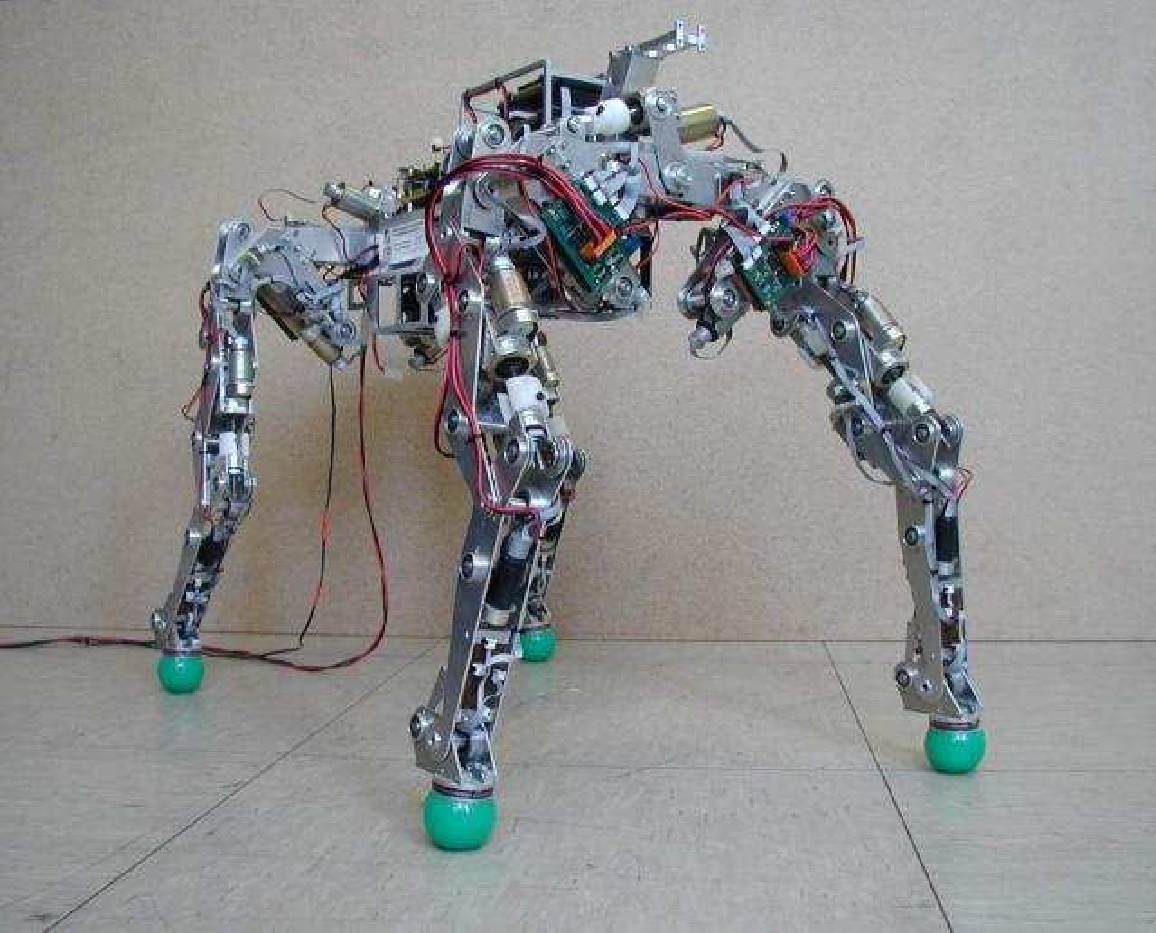
\includegraphics[width=5cm]{bisam}
       \caption{The quadrupedal walking machine Bisam developed at the Research Center
       for Information Technology in Karlsruhe.}
       \label{fig:bisam}
     \end{center}
   \end{figure}
\end{verbatim}
is used. This generates the output seen in~\ref{fig:bisam}.

\begin{figure}
  \begin{center}
    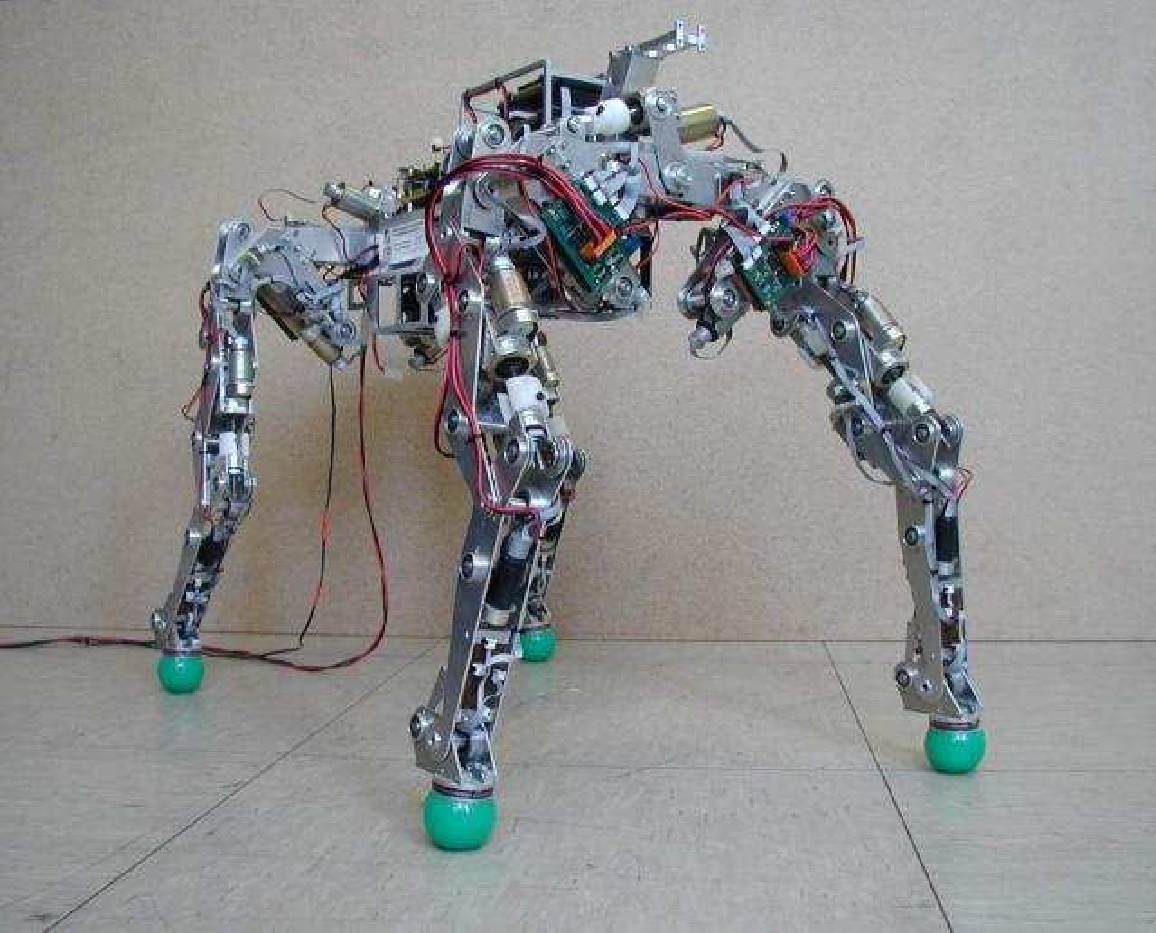
\includegraphics[width=5cm]{bisam}
    \caption{The quadrupedal walking machine Bisam developed at the Research Center
    for Information Technology in Karlsruhe.}
    \label{fig:bisam}
  \end{center}
\end{figure}

Specific commands and their parameters are referenced in appropriate literature. It's crucial that the image caption accurately describes what the image depicts. However, discussions about what's shown should be within the main text. For instance, if the figure is a plot, the caption might read: "Temperature trend with closed Valve B. Here, the temperature exceeds the critical limit at $t=\unit[130]{sec}$." The explanation of why this occurs, what effects are at play, or whether it's good or bad should not be under the image but discussed in the text. For data plots, ensure that all axes are properly labeled, and the legend is complete.

\begin{figure}
  \begin{subfigure}[b]{.5\linewidth}
    \centering 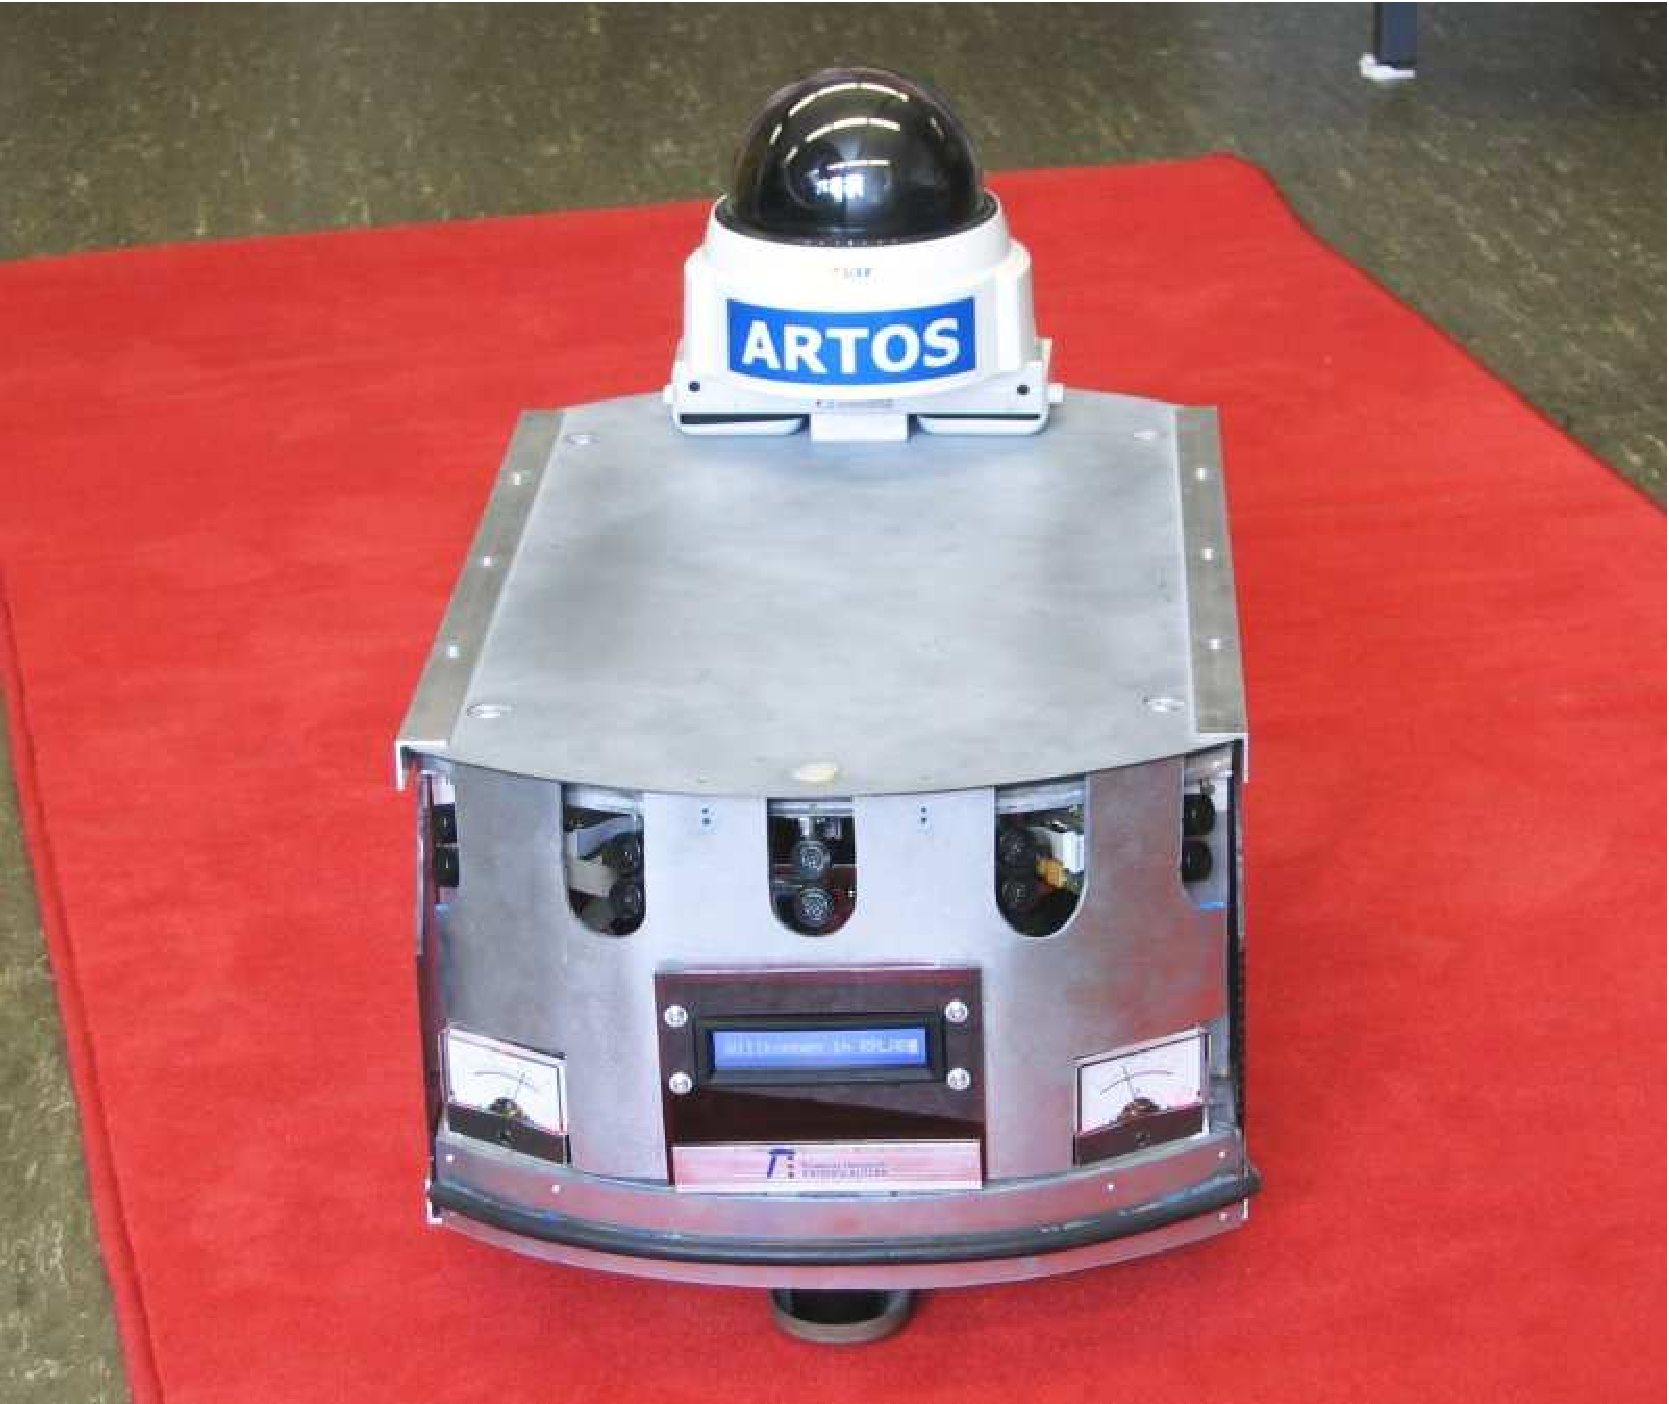
\includegraphics[height=5cm]{images/roter_teppich}
    \caption{\RRLABartos}
    \label{subfig:artos}
  \end{subfigure}%
  \hspace{1cm}
  \begin{subfigure}[b]{.5\linewidth}
    \centering 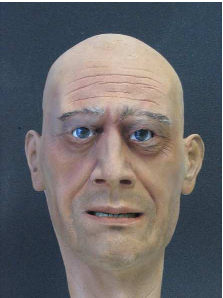
\includegraphics[height=5cm]{images/roman_mask}
    \caption{\RRLABroman}
    \label{subfig:roman}
  \end{subfigure}
  \caption{The mobile robot artos \RRLABartos (Autonomous Robot for Transport and Service)
  \subref{subfig:artos}  and the humanoid robot \RRLABroman (RObot huMAN interaction machine)
  \subref{subfig:roman}.}
  \label{fig:artos_and_roman}
\end{figure}

To include multiple images within a float environment, use something similar to:
\begin{verbatim}
\begin{figure}
  \begin{subfigure}[b]{.5\linewidth}
    \centering 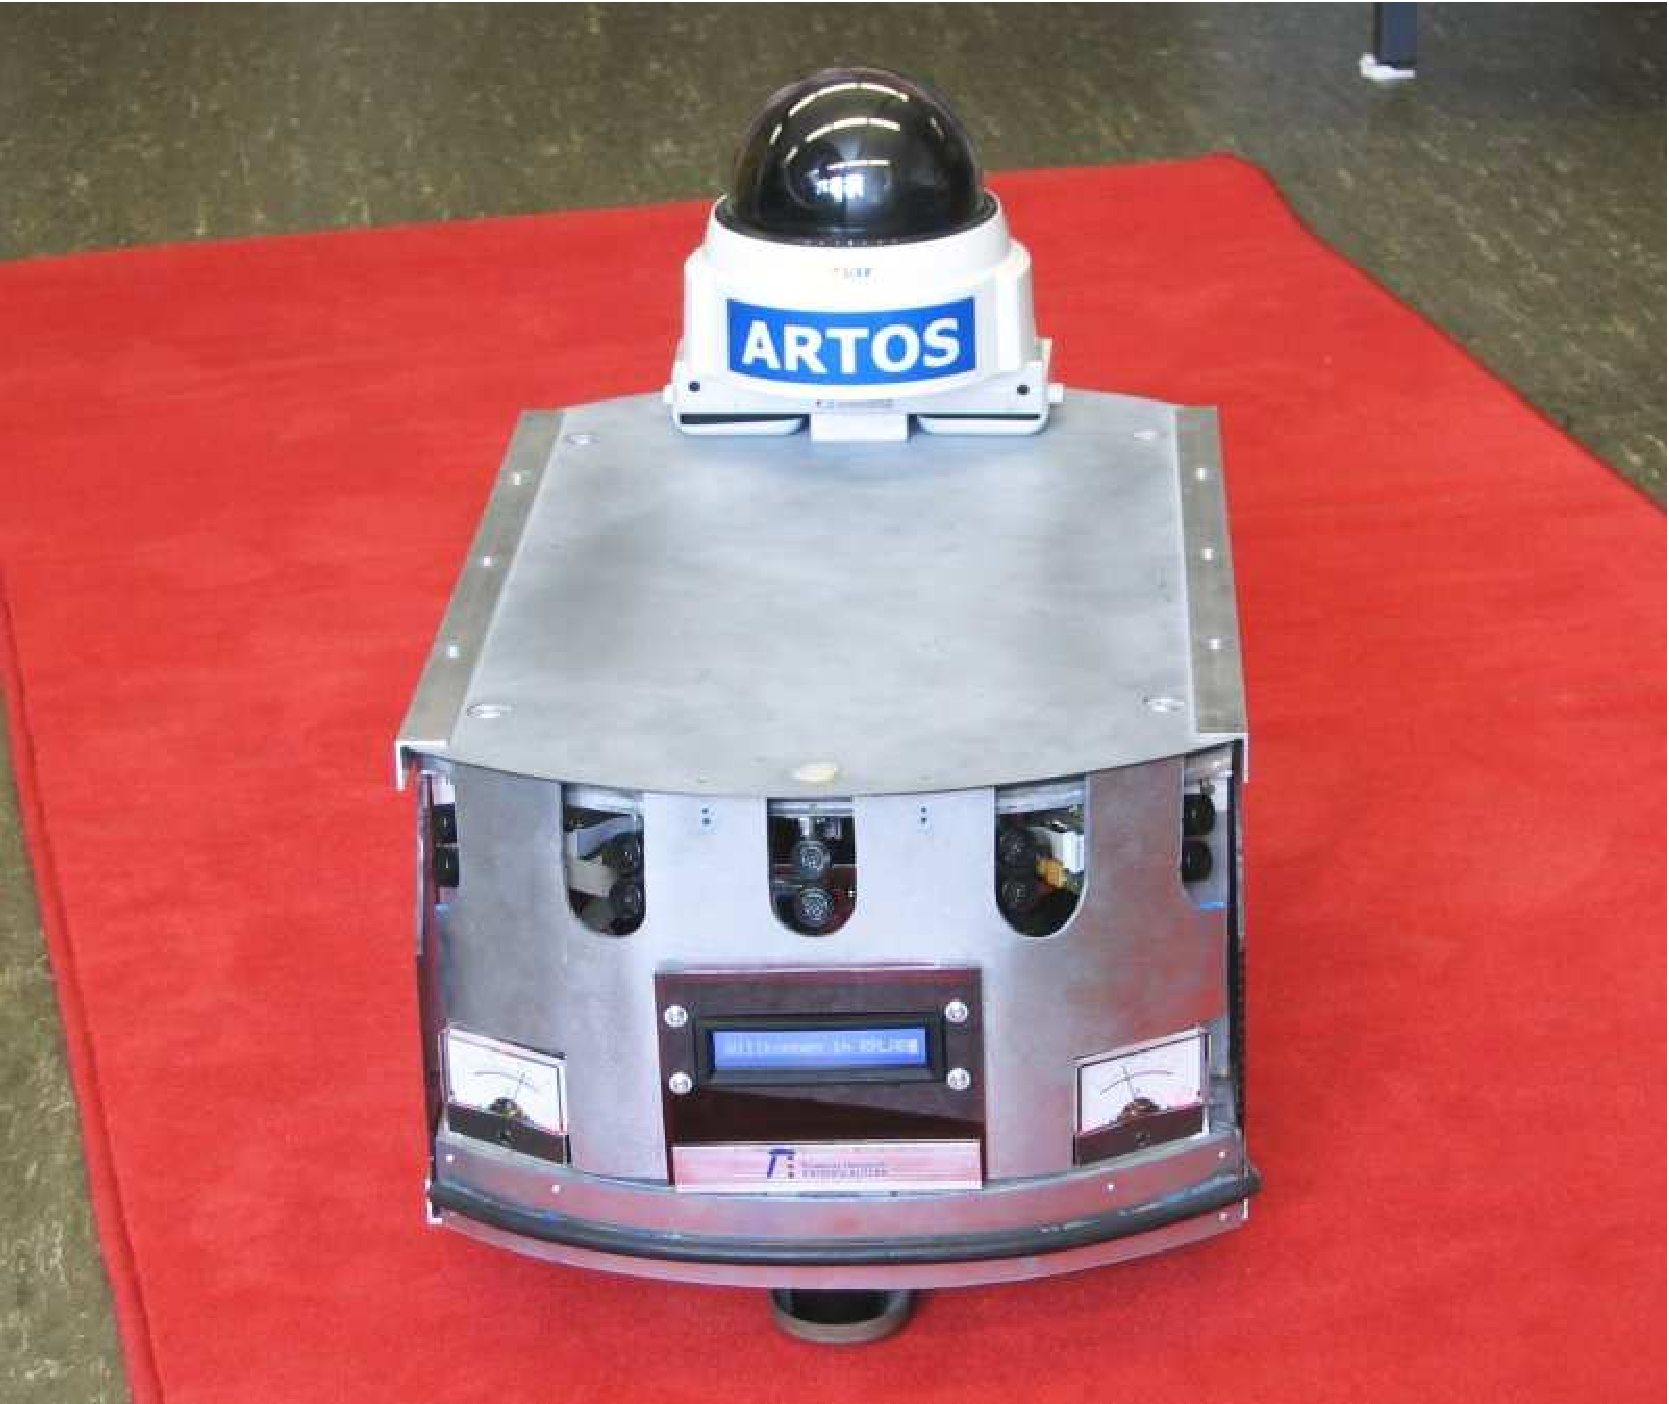
\includegraphics[height=5cm]{images/roter_teppich}
    \caption{\RRLABartos}
    \label{subfig:artos}
  \end{subfigure}%
  \hspace{1cm}
  \begin{subfigure}[b]{.5\linewidth}
    \centering 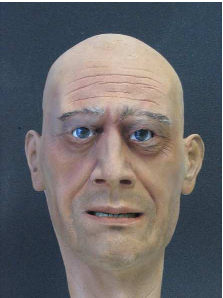
\includegraphics[height=5cm]{images/roman_mask}
    \caption{\RRLABroman}
    \label{subfig:roman}
  \end{subfigure}
  \caption{The mobile robot artos \RRLABartos (Autonomous Robot for Transport and Service)
  \subref{subfig:artos}  and the humanoid robot \RRLABroman (RObot huMAN interaction machine)
  \subref{subfig:roman}.}
  \label{fig:artos_and_roman}
\end{figure}
\end{verbatim}

This generates the output seen in Figure~\ref{fig:artos_and_roman}.

Alternatively, a ,,minipage'' can be used, as in Figures~\ref{fig:ARTOS} and~\ref{fig:ROMAN}. The ,,subfig'' variant is suitable when images are closely related and meant to be referenced as a single figure. The "minipage" is practical when both images are referenced separately.

\begin{figure}
  \begin{center}
    \begin{minipage}{0.48\textwidth}
      \begin{center}
        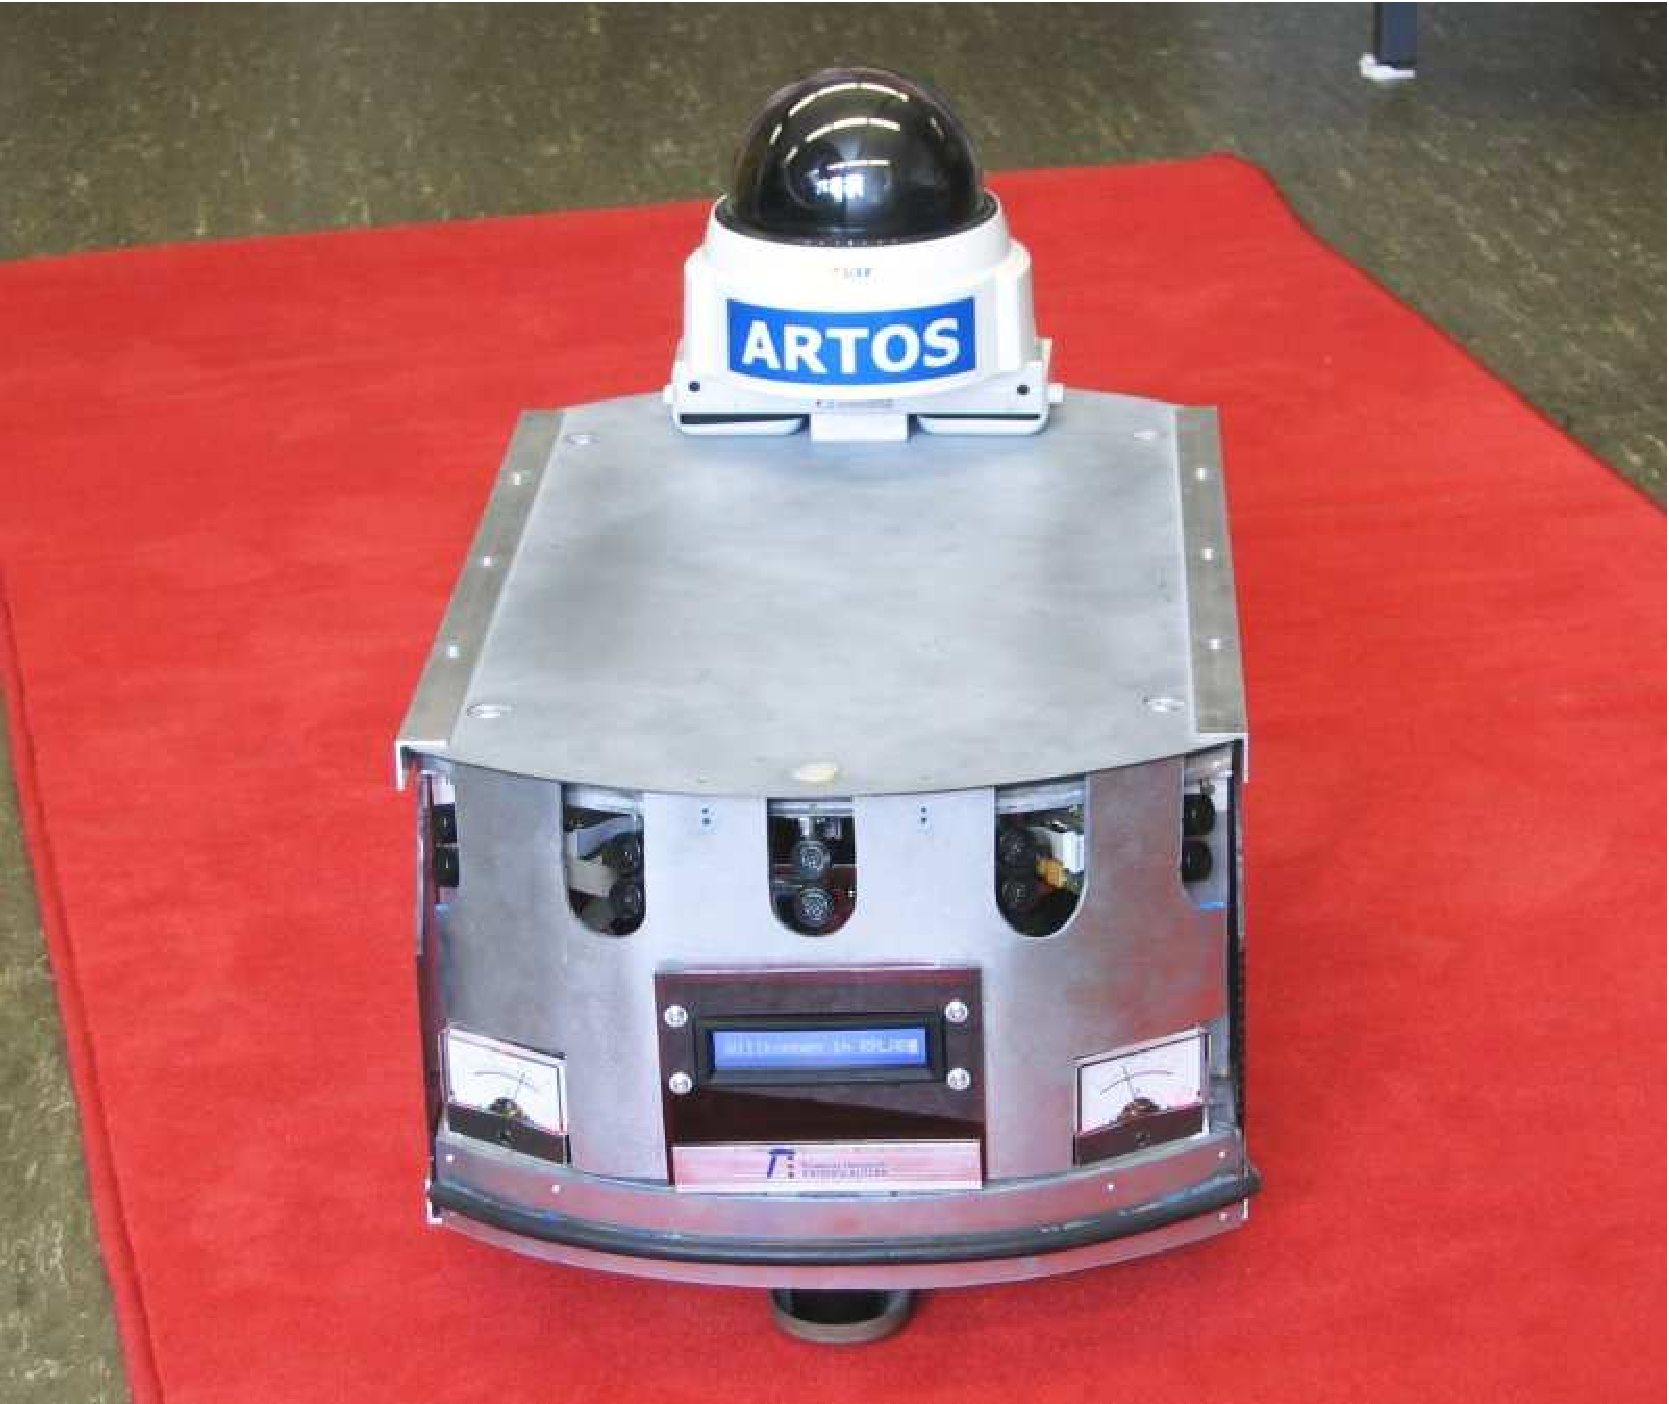
\includegraphics[height=5cm]{images/roter_teppich}
        \caption{Der mobile Roboter \RRLABartos (Autonomous Robot for Transport and Service).}
        \label{fig:ARTOS}
      \end{center}
    \end{minipage}
    \hspace{0.02\textwidth}
    \begin{minipage}{0.48\textwidth}
      \begin{center}
        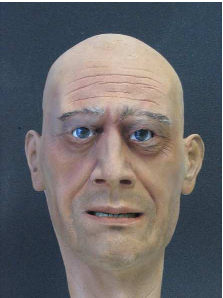
\includegraphics[height=5cm]{images/roman_mask}
        \caption{Der humanoide Roboter \RRLABroman (RObot huMAN interaction machine).}
        \label{fig:ROMAN}
      \end{center}
    \end{minipage}
  \end{center}
\end{figure}

The associated source code would look like this:

\begin{verbatim}
\begin{figure}
  \begin{center}
    \begin{minipage}{0.48\textwidth}
      \begin{center}
        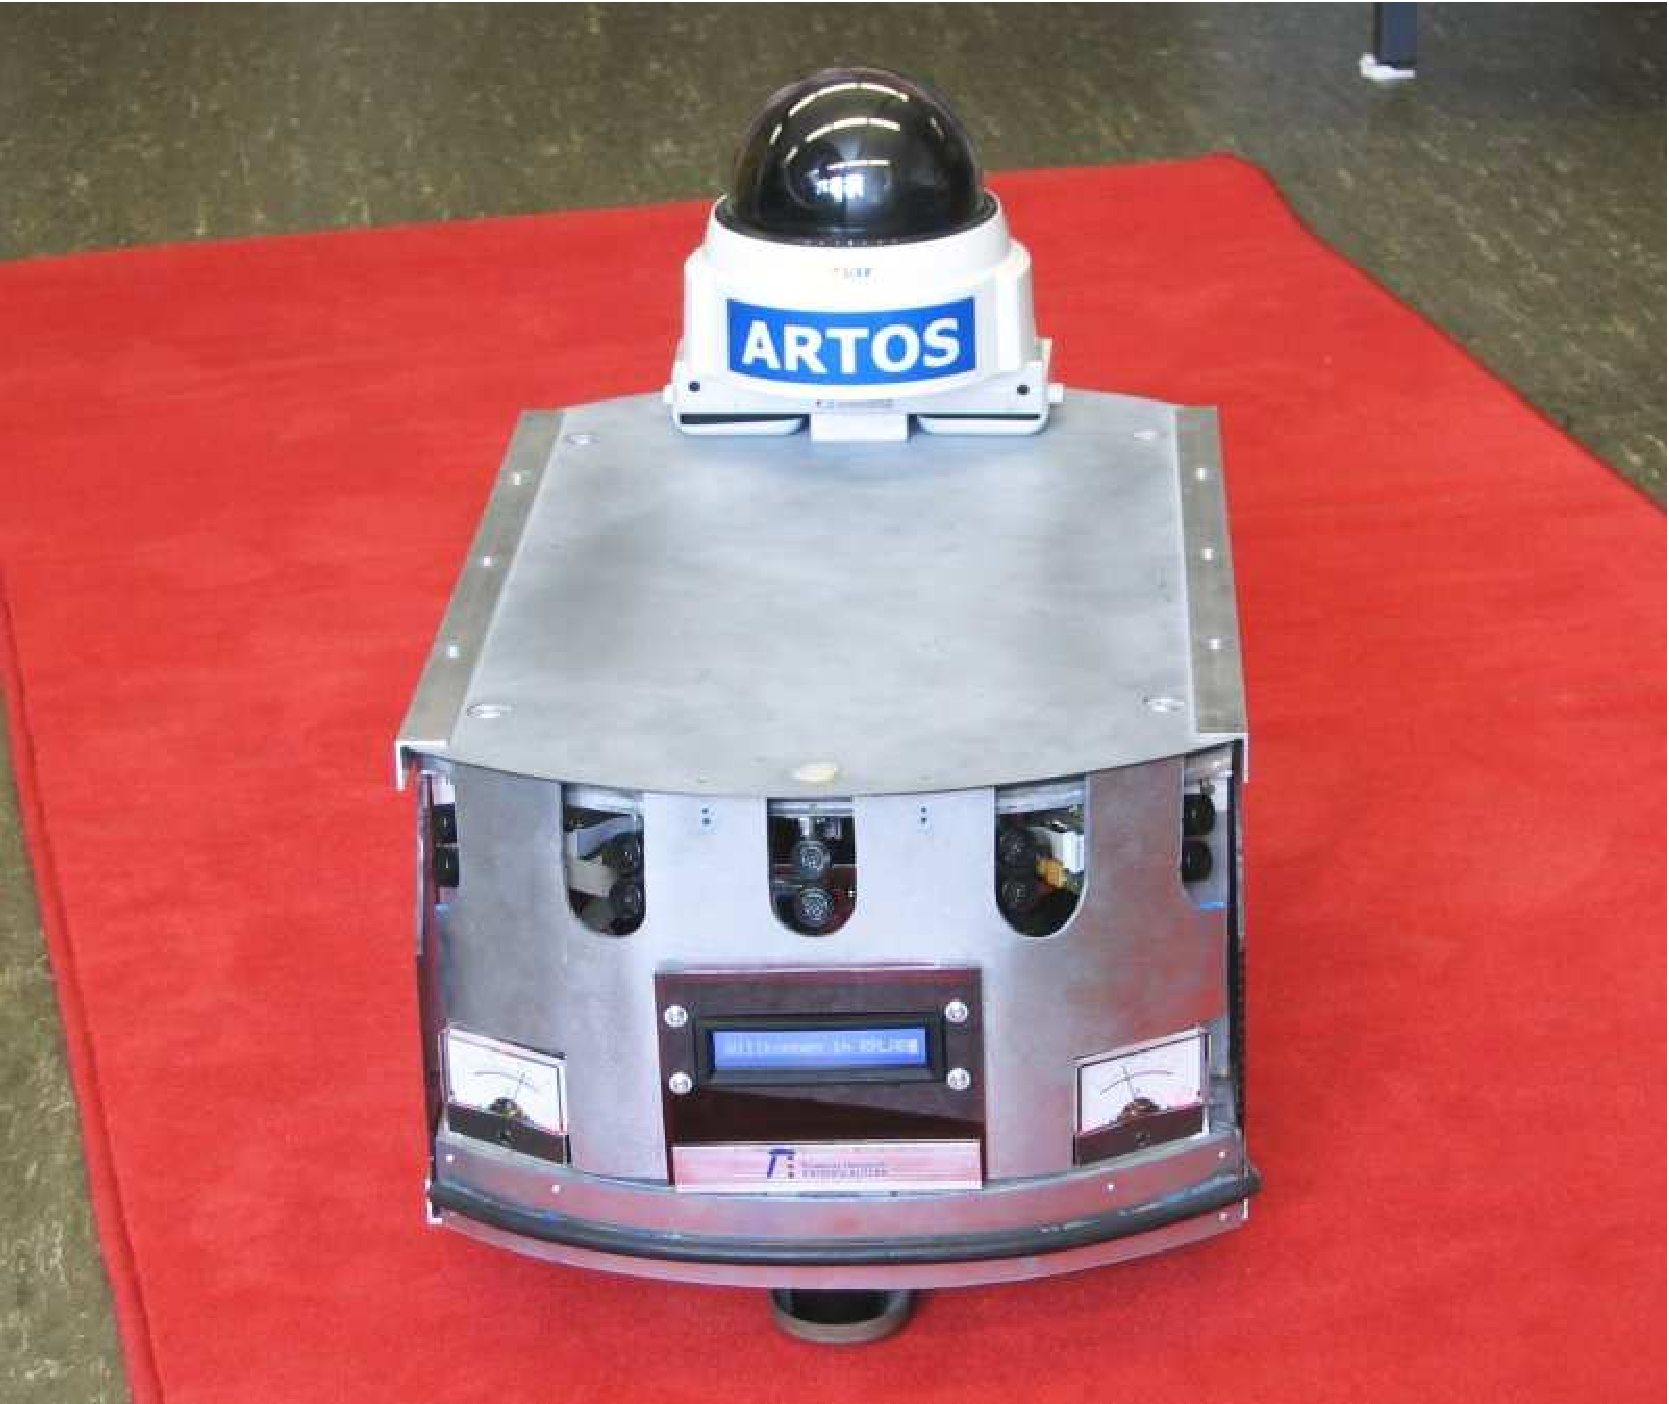
\includegraphics[height=5cm]{images/roter_teppich}
        \caption{Der mobile Roboter \RRLABartos 
            (Autonomous Robot for Transport and Service).}
        \label{fig:ARTOS}
      \end{center}
    \end{minipage}
    \hspace{0.02\textwidth}
    \begin{minipage}{0.48\textwidth}
      \begin{center}
        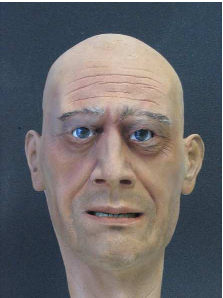
\includegraphics[height=5cm]{images/roman_mask}
        \caption{Der humanoide Roboter \RRLABroman 
            (RObot huMan interAction machiNe).}
        \label{fig:ROMAN}
      \end{center}
    \end{minipage}
  \end{center}
\end{figure}
\end{verbatim}


%%%%%%%%%%%%%%%%%%%%%%%%%%%%%%%%%%%%%%%%%%%%%%%%%%%%%%%%%%%%
\section{Tables}
\label{sec:floats:tables}
\index{Tables}The principles regarding the captioning of tables are similar to those for images. One can experiment with the number of lines, but the table appearance should remain consistent throughout the document. Table~\ref{tab:files} can serve as an example of tables.

%%%%%%%%%%%%%%%%%%%%%%%%%%%%%%%%%%%%%%%%%%%%%%%%%%%%%%%%%%%%
\section{Formulas und Units}
\label{sec:floats:formulas}
\index{Formulas} Formulas shouldn't get lost within the text, even if they're small (and unimaginative), such as $E=mc^2$, but rather be displayed in an \verb|equation| environment like so:
\begin{equation}
  \label{eq:einstein}
  E=mc^2 
\end{equation}
Generally, formulas should be numbered. For longer derivations, it suffices to label only important steps and the final result. When variables are mentioned in the text, such as the energy $E$ or the speed of light $c$ from Equation~\ref{eq:einstein}, these should be in math mode (e.g., \verb|$E$|). For complex formulas, the ,,amsmath'' package is included in the template. To display values with units, the ,,\verb|\unit|'' command is used, e.g., \unit[5]{mm} or \unitfrac[100]{km}{h} are generated using \verb|\unit[5]{mm}| or\ \verb|\unitfrac[100]{km}{h}|. If using the Euro symbol, include the ,,eurosym'' package.

%%%%%%%%%%%%%%%%%%%%%%%%%%%%%%%%%%%%%%%%%%%%%%%%%%%%%%%%%%%%
\section{Algorithms}
\label{sec:floats:algo}
\index{Algorithms} To visualize algorithms and special program sections, the functionality of the \verb|algorithm2e.sty| package can be employed. Both are supported, for instance, in \cite{WWWDante}, but generally aren't included in \LaTeX distributions, which is why we provide them.

\begin{algorithm}
  Create a 2D array\\
  Perform depth-first search:\\
\ForAll{nodes of tree U with coordinates $(x,y,z)$}{%
  \If{$z$-coordinate  of cell is greater than value in array at $(x,y)$}
    {Store $z$ at position  $(x,y)$ in 2D array}
}
Create Quadtree $G$\\
Perform depth-first search again:\\
\ForAll{nodes of tree $U$ with coordinates $(x,y,z)$}{%
  \If{coordinates match those stored in the 2D array}
    {Store $z$ for $(x,y)$ in Quadtree $G$}
}
\caption{Generating a global 2D map $G$ from an original map $U$}
\label{alg:example}
\end{algorithm}

The file \verb|algorithm2e.pdf| is attached as documentation. Generally, significant algorithms should be represented in pseudocode similar to Algorithm~\ref{alg:example} using these packages to enhance understanding. If it's necessary to include ,,actual'' source code (which mostly belongs in the appendix), the \LaTeX style \verb|listings.sty| is recommended, refer to Chapter~\ref{sec:floats:source_code}

Als Dokumentation ist die Datei  beigef\"ugt. Grunds\"atzlich
sollten wichtige Algorithmen als Pseudocode in der Art von
Algorithmus mithilfe dieser Pakete angegeben
werden, um das Verst\"andnis zu erleichtern. Sollte es tats\"achlich n\"otig
sein, ,,richtigen'' Quellcode einzuf\"ugen (der aber h\"ochstens mal in
den Anhang geh\"ort), ist der \LaTeX -Style \verb|listings.sty|
empfehlenswert, Kapitel~\ref{sec:floats:source_code}.


%%%%%%%%%%%%%%%%%%%%%%%%%%%%%%%%%%%%%%%%%%%%%%%%%%%%%%%%%%%%
\section{References}
\label{sec:floats:bib}
\index{References} All sources used must be listed in the bibliography, and references to them should be made at the corresponding text location. This is done with \verb|\cite{<label>}|, where \verb|<label>| corresponds to the entry in the BibTeX file. The name of the BibTeX file is passed to the \verb|literatur| macro in the main document (also refer to Chapter~\ref{sec:class:main}). For guidance on constructing the BibTeX file, take a look at \verb|literatur.bib| or consult appropriate literature (\cite{Lamport95}, \cite{WWWBibTex}). Additionally, examples for most possible BibTeX entries and explanations can be found in the file \verb|examples.bib|. Below are examples of the most important types:

\begin{itemize}
 \item Article in a journal~\cite{Albiez03}
 \item Book~\cite{Arkin98}
 \item Thesis~\cite{Luksch02}
 \item Dissertation~\cite{Breazeal00}
 \item Chapter in a Book~\cite{Mendel70}
 \item Chapter in a Collection~\cite{Ilg99}
 \item Conference proceedings~\cite{Berns07}
 \item Conference paper~\cite{Berns06}
 \item Technical report~\cite{Schaefer03}
\end{itemize}

The BibTeX layout generates references consisting of the last name of the first author and the last two digits of the publication year. When referencing URLs, the \verb|@Misc| entry can be used as demonstrated in \verb|literatur.bib|. As internet pages are subject to dynamic changes, they are not suitable for citing and referencing like books. Therefore, footnotes are a popular alternative for referencing internet pages.\footnote{http://rrlib.cs.uni-kl.de/}.


%%%%%%%%%%%%%%%%%%%%%%%%%%%%%%%%%%%%%%%%%%%%%%%%%%%%%%%%%%%%
\section{Index}
\label{sec:floats:index}
\index{Index} In larger works, creating an index can be useful. It's advisable to plan this from the start, making it easy to add index references at interesting points. This is done using \verb|\index{<keyword>}|, listing the <keyword> in the index directory along with the page number where the index command is located. Subpoints can be created with \verb|\index{<keyword>!<subpoint>}|. The index itself can be generated in the main document using the following macro: \verb|\RRLABindex|.

%%%%%%%%%%%%%%%%%%%%%%%%%%%%%%%%%%%%%%%%%%%%%%%%%%%%%%%%%%%%
\section{Additional Notes}
\index{Punctuation}
\index{Enumerations}

The ,,\verb|\itemize|'' environment is used for creating lists. Further instructions on punctuation are explained below:

\begin{itemize}
 \item If there isn't a complete sentence, start with lowercase after the bullet point.
 \item If a complete sentence follows a colon, start with a capital letter.
 \item No spaces are added before~.~,~!~?~:~;~,~etc.
 \item Quotation marks in German look like ,, (generated as \verb|,,|) while in English they appear  as `` (generated as \verb|``|).
 \item The closing quotation marks in both German and English look like '' (generated as \verb|''|).
 \item  There are four types of dashes: - (generated as \verb|-|), -- (generated as \verb|--|), --- (generated as \verb|---|) and $-$ (generated as \verb|$-$|). 

 The first is used as a hyphen, en dash, or em dash. In German, words consisting of several nouns are written together or alternatively separated by hyphens. In English, hyphens are omitted. For example:
 Mensch"=Roboter"=Interaktion bzw.\ human-robot interaction in English. Additionally, words composed of both English and German words are hyphenated. 

 The second dash is used as an em dash in German and for ranges and compound words.

 The third is used as an em dash in English and for tables. In German, spaces are added before and after the dash; in English, they are not (,,Du magst ja recht haben -- aber ich sehe das ganz anders.'' "the fire drill---it was chaos'').


 The last dash is the minus sign.
 
 \item Regarding number representation, there are several methods: traditionally, numbers from 0--11 are written as words, but newer conventions allow all numbers to be written as digits. Whichever style is chosen, consistency is key. 
\end{itemize}

If using the German language package, a hyphen determines where a word can be split (only at that point). This can lead to problems with compound words (e.g., Mensch"=Roboter"=Interaktion). To avoid this issue, hyphens can be coded as follows: \verb|Mensch"=Roboter"=Interaktion|. When referencing a webpage, it's best to do so with a footnote\footnote{\url{http://agrosy.informatik.uni-kl.de/}}. The code looks like: \verb|\footnote{\url{http://agrosy.informatik.uni-kl.de/}}|.


%%%%%%%%%%%%%%%%%%%%%%%%%%%%%%%%%%%%%%%%%%%%%%%%%%%%%%%%%%%%
\section{Darstellen von Quellcode-Fragmenten}
\label{sec:floats:source_code}
\index{Quellcode}

For C++ code, the following can be used:

\begin{verbatim}
\lstloadlanguages{C++}
\lstset{language=[GNU]C++, basicstyle=\tiny, breakautoindent,
breaklines, deletekeywords={LOCAL_DEBUG, MODULE_DEBUG, \#undef},
keywordstyle=\textbf, commentstyle=\color{Gray}, alsoletter=
{\#, \"}, emph={bool, byte, short, int, long, float, double, 
long double, char, const, static}, emphstyle=\color{red}, 
stringstyle=\color{red}, morecomment=[l][\color{green}]{\#}, 
numberstyle=\color{blue}, morecomment=[s][\color{blue}]
{/*}{*/}} 
\begin{lstlisting} 
  .
  .
  .
\end{verbatim}

This will render it relatively similar to how it appears in kdevelop.

\lstloadlanguages{C++}
\lstset{language=[GNU]C++, basicstyle=\tiny, breakautoindent, breaklines, deletekeywords={LOCAL_DEBUG, MODULE_DEBUG, \#undef},keywordstyle=\textbf, commentstyle=\color{Gray}, alsoletter={\#, \"}, emph={bool, byte, short, int, long, float, double, long double, char, const, static}, emphstyle=\color{red}, stringstyle=\color{red}, morecomment=[l][\color{green}]{\#}, numberstyle=\color{blue}, morecomment=[s][\color{blue}]{/*}{*/}}

\begin{lstlisting} 
// this is a -*- C++ -*- file
//----------------------------------------------------------------------
/*!\file    mbbDrive.C
 *
 * \author   Jochen Hirth
 * \date    18.04.06
 *
 * $Revision: 1.3 $
 * $Id: NullBehaviourBasedModule.C,v 1.3 2005/10/04 11:17:39 martin Exp $
 *
 */ 
//----------------------------------------------------------------------
// Includes
//----------------------------------------------------------------------

#include "mbbDrive.h"

//----------------------------------------------------------------------
// Module Debug
//----------------------------------------------------------------------
//#undef MODULE_DEBUG
#define MODULE_DEBUG
#include "kernel/ModuleDebug.h"

//----------------------------------------------------------------------
// Debugging
//----------------------------------------------------------------------
#undef LOCAL_DEBUG 
//#define LOCAL_DEBUG
#include "kernel/LocalDebug.h"

//----------------------------------------------------------------------
// defines and consts
//----------------------------------------------------------------------

//----------------------------------------------------------------------
// class mbbDrive constructor
//----------------------------------------------------------------------
mbbDrive::mbbDrive( tParent *parent, tDescription name, tBehBBHandler* _beh_bb_handler, bool fixit )
        : tBehaviourBasedModule( parent, name,
                                 eSI_DIMENSION, eSO_DIMENSION, eCI_DIMENSION, eCO_DIMENSION,
                                 si_description, so_description, ci_description, co_description, _beh_bb_handler )
{

    sigmoid = new tSigmoid( tSigmoid::eSIG_RISE, 0., 1. );
}

//----------------------------------------------------------------------
// class mbbDrive destructor
//----------------------------------------------------------------------
mbbDrive::~mbbDrive()
{
    delete sigmoid;
}

\end{lstlisting}

However, you can also load the code or selected lines from a file and display line numbers:

\begin{verbatim}
\lstinputlisting[numbers=left,linerange={1-4,7-26}]{mbbDrive.cpp}
\lstinputlisting[numbers=left,linerange={33-43}]{mbbDrive.cpp}
\end{verbatim}

Und das sieht dann so aus:

\lstinputlisting[numbers=left,linerange={1-4,7-26}]{mbbDrive.cpp}
\lstinputlisting[numbers=left,linerange={33-43}]{mbbDrive.cpp}

For \textsc{xml}-code, the following setting is appropriate:

\begin{verbatim}
\lstset{language=xml, basicstyle=\tiny, breakautoindent,
 breaklines,keywordstyle=\textbf, keywordsprefix=<, 
identifierstyle=\color{green}, stringstyle=\color{red}} 
\begin{lstlisting} 
  .
  .
  . 
\end{verbatim}

The output will look like this:

\lstset{language=xml, basicstyle=\tiny, breakautoindent, breaklines, keywordstyle=\textbf, keywordsprefix=<, identifierstyle=\color{green}, stringstyle=\color{red}}

\begin{lstlisting} 
<?xml version="1.0" encoding="ISO-8859-1"?>
<data xmlns:xsi="http://www.w3.org/2001/XMLSchema-instance"
 xsi:schemaLocation="Belami DoAmi_dialog_description_scheme(v1.2).xsd"
 xmlns:belami="http://www.w3.org/2001/Belami"
 xmlns="http://www.w3.org/2001/Belami">
    <platform type="desktop">
        <SUI_settings>
            <tts_settings context="free" voice="0" speed="100" activate="immediately"/>
            <asr_settings activate="immediately" timeout="4" acknowledge="true"/>
        </SUI_settings>	       
	<dialog dialog_id="Welcome">
		<SUI_dialog>
	    	<SUI_settings>
                </SUI_settings>
			<prompt>Hallo! Ich bin Roman, der humanoide Roboterkopf der technischen Universiteet Kaiserslautern. Meine Aufgabe ist es, mit Menschen zu kommunizieren. Hierzu kann ich emotionale Gesichtsausdruicke einsetzen.</prompt>
			<goto mark="Recognize"/>
	</SUI_dialog>
        </dialog>

\end{lstlisting}

Additionally, the "listings" package offers the ability to display many other programming languages. For more information, please refer to the accompanying documentation.

%%% Local Variables: 
%%% mode: latex
%%% TeX-master: "howto"
%%% End: 


%%%%%%%%%%%%%%%%%%%%%%%%%%%%%%%%%%%%%%%%%%%%%%%%%%%%%%%%%%%%
%% introduction.tex
%%
%% Kapitel: Introduction
%% Autor: Axel Vierling (axel.vierling@cs.rptu.de)       
%% Autor: Jochen Hirth (j_hirth@informatik.uni-kl.de)       
%% Autor: Tobias Luksch (luksch@informatik.uni-kl.de)       
%% Datum: Juli 2003                                         
%%                                                          
%% Letzte Änderung Dezember 2023
%%%%%%%%%%%%%%%%%%%%%%%%%%%%%%%%%%%%%%%%%%%%%%%%%%%%%%%%%%%%
\chapter{Structure of the Document}
\label{chap:structure}
Here are some guidelines and recommendations to consider when creating the document. This section focuses more on the structural organization of the work rather than syntactical issues as addressed previously.

Foremost recommendation: It's crucial to consult with your supervisor early and frequently, especially regarding aspects like the structure and actual scientific content. This approach might save you some effort and time and provide assurance that you are on the right track, avoiding potential misdirection.

%%%%%%%%%%%%%%%%%%%%%%%%%%%%%%%%%%%%%%%%%%%%%%%%%%%%%%%%%%%%
\section{Thesis}
\label{sec:structure:thesis}
The most common structure of a thesis, valid for both master or bachelor theses usually looks like this
\begin{itemize}
    \item Introduction --- Here the topic should be introduced, and the structure, goal and scope of the thesis should be defined. One should focus on answering the following question: Why is the topic of the Thesis interesting for the (scientific) community?
    \item Background --- The main focus of this chapter should be to introduce everything that is needed to understand the further concepts of the thesis. This should entail everything you had to learn to understand and implement the task, and shortly cover the courses in your specialization you needed to understand the topic. The goal is to enable a reader from the same study program potentially from another specialization to understand the thesis.
    \item Related Work --- This question should answer the question: How did others try to solve the problem, and what did they miss? So, why is the problem not yet solved? In short, this should define the research gap of your work. For this, state-of-the-Art approaches should be described.
    \item Concept \& Implementation --- This is the first main part of the thesis. Here the approach you and your supervisor decided on should be explained. Usually, first on a higher level and then in detail including implementation details. So the question that is answered is: How do you try to solve the problem at hand?
    \item Experiments --- This is the second main part of the thesis. The experiments should be suitable to validate your approach. Define the experimental setting, e.g. the robot or the dataset, the metrics as well as the results. The visualization of the results should be in a way such that it is easily understandable. Usually, first, the results are reported and then the effects of the results on the defined problem are discussed. Answer the question, what parts of the problem did you solve?
    \item Conclusion \& Future Work --- Here the approach should be discussed related to the initial scope and goal. Answer the questions: What did you solve and especially what did you \textbf{not} solve? Give hints for potential extensions as future work.
\end{itemize}

%%%%%%%%%%%%%%%%%%%%%%%%%%%%%%%%%%%%%%%%%%%%%%%%%%%%%%%%%%%%
\section{Project}
\label{sec:structure:project}
The structure of a project is usually quite similar to the thesis, see Section~\ref{sec:structure:thesis}. As the scope is smaller, the Background and Related Work chapters are combined into one. But the exact structure depends more strongly on the task of the project.

%%%%%%%%%%%%%%%%%%%%%%%%%%%%%%%%%%%%%%%%%%%%%%%%%%%%%%%%%%%%
\section{Seminar}
\label{sec:structure:seminar}
The structure of the seminar again depends greatly on the topic -- and the supervisor. Here is however a general concept. Again, it is somewhat similar to Section~\ref{sec:structure:thesis}
\begin{itemize}
    \item Introduction --- Here the topic should be introduced, and the structure, goal and scope of the thesis should be defined. One should focus on answering the following question: Why is the topic of the Thesis interesting for the (scientific) community?
    \item Background --- The main focus of this chapter should be to introduce everything that is needed to understand the further concepts of the thesis. This should entail everything you had to learn to understand and implement the task, and shortly cover the courses in your specialization you needed to understand the topic. The goal is to enable a reader from the same study program potentially from another specialization to understand the thesis.
    \item State-of-the-Art Overview --- Answer the following questions: What different approaches exist to solve the problem? What do they do similar? What are the differences? What is the remaining research gap? All of this should be answered concisely, often best in a table. This should give a broad overview of the papers you read in your initial phase and summarize the overall topic. 
    \item Detailed-Concepts --- Here usually one or two approaches should be discussed in detail. Describe the key elements and how they solve the problem. More then 2 approaches can not be discussed in enough detail.
    \item Conclusion --- Here the results of the seminar should be summarized.
\end{itemize}

Instead of the here presented Top-Down approach also a Bottom-Up seminar report can be done, where chapters 3 and 4 are swapped.

\section{Dissertation}
\label{sec:structure:dissertation}
See Figure~\ref{fig:diss_structure}

\begin{figure}
    \begin{center}
      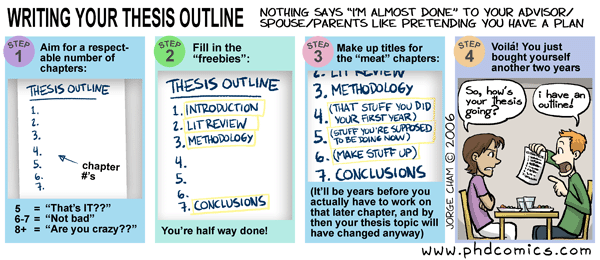
\includegraphics[width=15cm]{Diss_Structure}
      \caption{Common disserstation structure, see \url{https://phdcomics.com/comics/archive.php?comicid=715}}
      \label{fig:diss_structure}
    \end{center}
  \end{figure}


%%% Local Variables: 
%%% mode: latex
%%% TeX-master: "howto"
%%% End: 


\chapter{Another chapter}
\label{chap:addendum}

\section{Why this section and chapter?}
This chapter only exists to highlight, that it is possible
to use a mixture of directly inserted Text and files
that are included via \verb|\include|. For short documents
it might be more feasible to use only a single \LaTeX file,
as it is faster and easier to keep an overview.

%%%%%%%%%%%%%%%%%%%%%%%%%%%%%%%%%%%%%%%%%%%%%%%%%%%%%%%%%%%%
%% Bibliography
%%
%% Inclusion of the Bibliography. The macro expects
%% BibTex-Files (e.g. literature.bib) without file identifier
%% as a Parameter
%%%%%%%%%%%%%%%%%%%%%%%%%%%%%%%%%%%%%%%%%%%%%%%%%%%%%%%%%%%%
\RRLABbibliography{literatur}

%%%%%%%%%%%%%%%%%%%%%%%%%%%%%%%%%%%%%%%%%%%%%%%%%%%%%%%%%%%
%% Create Index, comment if not needed
%%%%%%%%%%%%%%%%%%%%%%%%%%%%%%%%%%%%%%%%%%%%%%%%%%%%%%%%%%%%
\RRLABindex

%%%%%%%%%%%%%%%%%%%%%%%%%%%%%%%%%%%%%%%%%%%%%%%%%%%%%%%%%%%%
%% End of the Document
%%%%%%%%%%%%%%%%%%%%%%%%%%%%%%%%%%%%%%%%%%%%%%%%%%%%%%%%%%%%
\end{document}
